\chapter{Oldalak}

\section{Új üzenet küldése}
\begin{flushleft}
    Ezen oldalon lehetséges új üzenet küldése, akár több címzettnek is, ahol megadható tárgy, és maga a tartalom akár formázottan is.
\end{flushleft}
\begin{minipage}[h]{0.3\textwidth}
    \begin{itemize}
       \item Címzett(ek)
       \item Tárgy
       \item Üzenet tartalma
    \end{itemize}
\end{minipage}%
\begin{minipage}[h]{0.7\textwidth}
    \begin{center}
        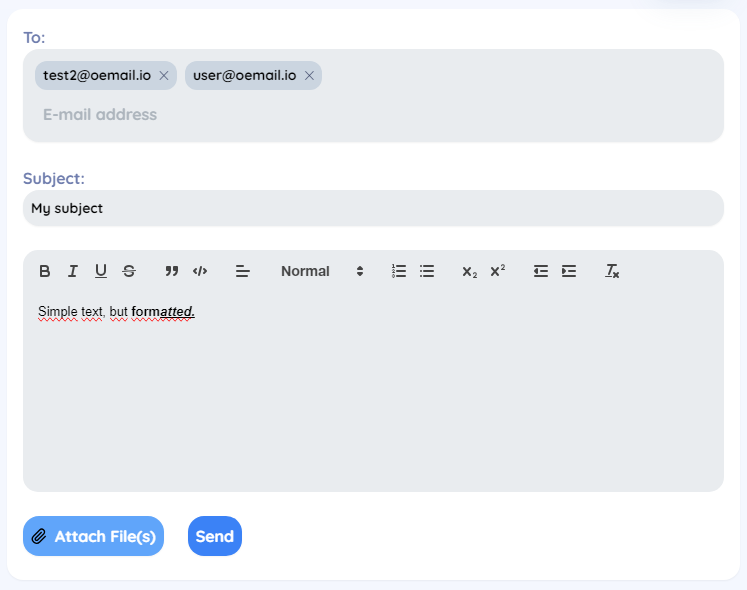
\includegraphics[width=1\textwidth]{send}
    \end{center}
\end{minipage}%

\section{Beérkezett üzenetek}
\begin{flushleft}
    A beérkezett üzenetek megtekintése ezen az oldalon található, ahol az adott üzenetet lehet törölni vagy csillagozni is.
\end{flushleft}
\begin{center}
    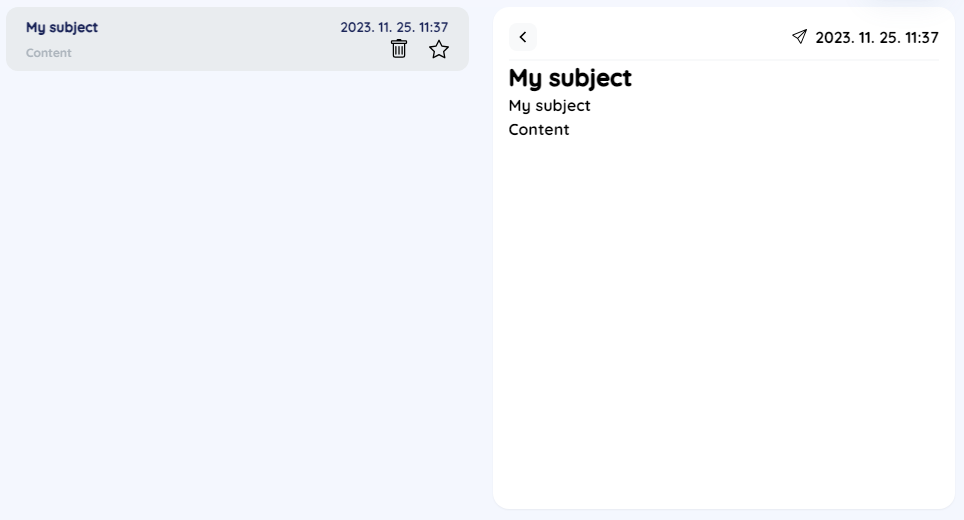
\includegraphics[width=0.8\textwidth]{message}
\end{center}

\section{Elküldött üzenetek}
\begin{flushleft}
    Itt találhatóak meg az elküldött üzenetek.
\end{flushleft}

\section{Szemét}
\begin{flushleft}
    Azok az üzenetek tárolódnak itt, amelyeket a felhasználó úgy vélt, hogy számára nem releváns, akkor azt a szemétbe is rakhatja.
\end{flushleft}

\section{Csillagozott}
\begin{flushleft}
    Felhasználó kedvenc, csillagozott levelei itt találhatóak meg.
\end{flushleft}

\section{Gyanús üzenetek - Spam}
\begin{flushleft}
    Ha van olyan beérkezett üzenet, amelyet a szoftver úgy vél, hogy gyanús lehet a felhasználóra tekintve, akkor azt itt található meg.
\end{flushleft}